\documentclass[12pt]{article}

% Packages
\usepackage[margin=1in]{geometry}
\setlength{\parindent}{0pt}
\usepackage{enumitem}

\usepackage{amsthm}
\theoremstyle{definition}
\newtheorem{example}{Example}[section]

\usepackage[normalem]{ulem}
\usepackage{censor}
\censorruledepth=-.2ex
\censorruleheight=.1ex
%\StopCensoring % Uncomment to fill in the blanks

\usepackage[colorlinks,urlcolor=blue,citecolor=black]{hyperref}

\usepackage{graphicx}
\graphicspath{ {Figures/} }







\begin{document}
% Chapter and section titles
\thispagestyle{empty}
\begin{center}
{\LARGE \bf Statistics, Inference, and Sampling}\\
{\large McCaig Statistics Group}\\
Bryce A. Besler
\end{center}

% % Objectives
% \section{Objectives}
% \begin{itemize}[itemsep=1pt]
%   \item Understand the terminology of experiments
%   \item Differentiate Correlation and Causation
%   \item Understand Sampling and Sampling Distributions
%   \item Define Parameters and Statistics and their relationship to inference
% \end{itemize}

% % Randomized Experiments
\section*{Experiments}
% Why would someone perform a study or an experiment?
% \begin{itemize}[itemsep=1pt]
%   \item \xblackout{We have questions and want answers!}
%   \item \xblackout{Experimentation is key to learning. (i.e. a child touching a hot burner)}
% \end{itemize}

The following examples are fictionalized for the purpose of differentiating randomized experiments from observational studies.

\begin{example}
\label{ex:gsa}
The Graduate Student Association (GSA) offers workshops on scholarship writing for students.
They are interested in how effective these workshops are at helping students secure funding.
In the last 5 years, 2198 students applied to national funding (NSERC, CIHR, SSHRC).
Of those students, 916 attended a workshop on scholarship writing.
The GSA is able to attain the amount of money each student was awarded in national funding.
They discover that students who attend the scholarhips workshop secure an average of \$5,680 more than their peers who do not attend the workshop.
They conclude that workshops are extremely effective at helping students secure funding.
\end{example}

Let's identify the information in Example~\ref{ex:gsa}. 
\begin{description}[leftmargin=!, labelwidth=\widthof{\bfseries Independant Variable},itemsep=1pt]
  \item[Sample Size] \xblackout{2198}
  \item[Researcher(s)] \xblackout{GSA}
  \item[Method] \xblackout{Review history of attending workshops and amount of money awarded in national competitions.}
  \item[Results] \xblackout{Students who attend workshops attain \$5,680 more than their peers on average.}
  \item[Independant Variable] \xblackout{Attending a workshop}
  \item[Dependant Variable] \xblackout{Scholarship funding}
  \item[Experimental Units] \xblackout{Graduate Students}
\end{description}

\pagebreak

\begin{example}
\label{ex:mtc_gender_pub}
The MTC is interested in increase the number of scholarships McCaig trainees are awarded.
The MTC randomly funds 41 trainees to attend a workshop on scholarship writing.
The remaining 40 trainee do not attend the workshop.
All trainees apply for national funding and report their award value to the MTC.
The MTC finds that there is no difference in the amount of funding secured by trainees who attended the workshop compared to those who do attend.
The MTC find that scholarship workshops have no effect on funding success and stops financially supporting the workshop.
\end{example}

Let's identify the information in Example~\ref{ex:mtc_gender_pub}. 
\begin{description}[leftmargin=!, labelwidth=\widthof{\bfseries Independant Variable},itemsep=1pt]
  \item[Sample Size] \xblackout{81}
  \item[Researcher(s)] \xblackout{MTC}
  \item[Method] \xblackout{Randomly send some students to the workshop and not others}
  \item[Results] \xblackout{Attending the workshop does not increase the amount of money awarded}
  \item[Independant Variable] \xblackout{Attending a workshop}
  \item[Dependant Variable] \xblackout{Scholarship funding}
  \item[Experimental Units] \xblackout{McCaig Trainees}
\end{description}

We have the following terminology for experiments:
\begin{description}[leftmargin=!, labelwidth=\widthof{\bfseries Experimental Unit},itemsep=1pt]
  \item[\censor{Experimental Unit}] The material that is assigned treatment.
  \item[\censor{Sample Size}] Number of experimental units.
  \item[\censor{Treatment}] The variables the researcher changes. Also called independant variable, exposure, explanatory variable, predictor variable, etc.
  \item[\censor{Outcome}] The variables the researcher measures. Also called response, dependant variable.
\end{description}

% \section{Correlation and Causation}
% Do you think scholarship workshops increase the amount of money students are awarded on average?
% \vspace{2.5cm}

% What are the differences between these two studies?
% \begin{description}[leftmargin=!,itemsep=1pt]
%   \item \censor{\textbf{Sample Size.} The GSA study has many more students}
%   \item \censor{\textbf{Assigning Treatment.} The MTC assigned some students to attend and others not}
%   \item \censor{\textbf{Population.} McCaig trainees are a subset of all graduate students}
% \end{description}

% Example~\ref{ex:gsa} is an example of a \uline{randomized experiment}.
% The researchers (MTC) were able to assign treatment (attending a workshop) to the experimental units (McCaig Trainees).
% \\
% \\
% Example~\ref{ex:mtc_gender_pub} is an example of an \uline{observational study}.
% The researchers (GSA) could not assign treatment (attending a workshop) to the experimental units (graduate students).
% \\
% \\
% In general, \textbf{causation can only be established from \censor{randomized experiments} (and not \censor{observational studies})}~\cite{ramsey2012statistical}.
% This is because randomization leads to a mixing of \underline{confounding variables} between treatment groups.
% Observational studies - where researchers do not control the assigmnet of treatment to experimental units - cannot establish causation because the effect of confounding variables cannot be ruled out.
% However, the results from the MTC study do not generalize to all graduate students because McCaig Trainees are not a random sample of all graduate students.
% \\
% \\
% A confounding variable is defined as as \textbf{a variable related both to the \censor{treatment} and the \censor{outcome}}.
% Confounding variables make it difficult to establish the outcome as being a direct consequence of treatment~\cite{ramsey2012statistical}.
% Below are some confounding variable diagrams.
% What are a few confounding variables for the diagrams below?

% \begin{figure}[h]
%   \label{fig:confounding_funding}
%   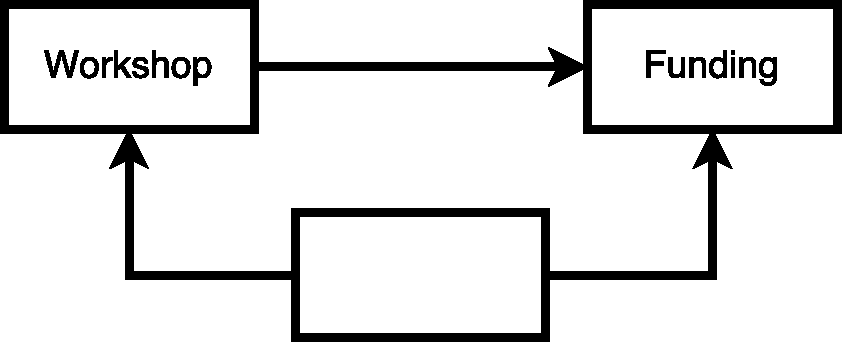
\includegraphics[width=12cm]{confounding_funding.pdf}
%   \centering
% \end{figure}
% \censor{Keen students, advertising strategy, gender, education, research training}

% \begin{figure}[h]
%   \label{fig:confounding_gender}
%   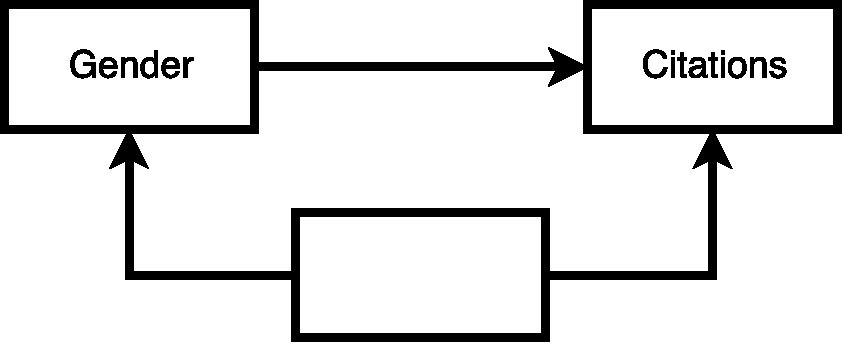
\includegraphics[width=12cm]{confounding_gender.pdf}
%   \centering
% \end{figure}
% \censor{Reviewer bias, education, family responsibilities}

% See \url{http://www.tylervigen.com/spurious-correlations} for examples of how confounding variables can lead you astray.

% \section{Parameters, Statistics, and Inference}
% We have discussed experiments.
% Now, we seek to answer our question (hypothesis) by using data from the experiment.
% That is, we seek to draw a \textbf{statistical inference}.
% Statistical inference is defined as 1) a conclusion that patterns in the data are present in some broader context and 2) the conclusion is justified by a probability model~\cite{ramsey2012statistical}.

% Consider the workshop experiment.
% From a population, a sample of 

% To do this, we first build a mathematical model.
% In the case of the workshop-funding examples, the model is that the mean of the outcomes is different.
% Let $\mu$ indicate the mean funding attained.
% \begin{eqnarray}
%   \mu_{ \textrm{workshop} } &\neq& \mu_{ \textrm{no workshop} }
% \end{eqnarray}

% This can be reduced to a single parameters $\delta$, the difference in average funding.
% \begin{eqnarray}
%   \textrm{Let } \delta &=& \mu_{ \textrm{workshop} } - \mu_{ \textrm{no workshop} } \\
%   \delta &\neq& 0
% \end{eqnarray}

% We call $\delta$ a parameter of the model.
% We can produce an estimate of the parameter, $\hat{\delta}$, denoted by the hat.
% $\hat{\delta}$ is called a statistic - an estimate of a parameter.
% Necessarily, the statistic is a random variable with a distribution because we have drawn a random sample.
% Consider a random sample $[x_1, x_2, ..., x_n]$.
% The statistics is random because the samples are random.
% \begin{eqnarray}
%   \hat{\delta} &=& f(x_1, x_2, ..., x_n)
% \end{eqnarray}


% \section{Sampling and Sampling Distributions}
% Why do we need to sample?
% Why can't we just measure everyone in the population?
% \begin{itemize}[itemsep=1pt]
%   \item \xblackout{Finite resources (time, money, materials, etc.)}
%   \item \xblackout{May be unethical (ACL transection of mice)}
% \end{itemize}

% Experimental design is the task of maximizing the amount of information attainable from limited resources.

% See \url{http://onlinestatbook.com/2/summarizing_distributions/balance.html} for a demonstration of sampling distributions.

% \section{Summary}
% \begin{description}[leftmargin=!, labelwidth=\widthof{\bfseries Confounding Variables}, itemsep=1pt]
%   \item[Terminology] Be familiar with language like \textbf{treatment}, \textbf{outcome}, and \textbf{experimental units}. 
%   \item[Causal Inference] Causal inference can only be drawn when the researcher assigns \blackout{treatment} to experimental units \censor{randomly}.
%   \item[Confounding Variables] A variable related both to the \blackout{treatment} and the \blackout{outcome}.
%   \item[Model] The mathematical formula implicit in the statistical test. The model contains parameters which are estimated by sampling the \censor{population distribution} and computing a \censor{statistics}.
%   \item[Sampling Distribution] The probability density function (or histogram or distribution) of a \censor{statistic} caused by sampling.
% \end{description}

% % Bibliography
% \bibliographystyle{ieeetr}
% \bibliography{references}

\end{document}
